\documentclass[english]{beamer}
\usetheme{Frankfurt}

\setbeamersize{description width=0.57cm}

\title{Finite temperature and $\delta$-regime in the Schwinger model}
\author{
  Ivan Hip\textsuperscript{a},
  Jaime Fabián Nieto Castellanos\textsuperscript{b},
  Wolfgang Bietenholz\textsuperscript{b}}
\institute{
  \textsuperscript{a}University of Zagreb, Croatia\\
  \textsuperscript{b}UNAM, Mexico
}
\date{July 29, 2021}

\begin{document}
 
\begin{frame}
  \titlepage
\end{frame}


\section{Introduction}

\begin{frame}{Schwinger model}
  \begin{itemize}
    \item introduced by [Schwinger, 1961]:
      \textit{two-dimensional quantum electrodynamics}
      --- fermions coupled to Abelian gauge field 
    \item simple example for chiral anomaly and confinement
    \item often used as a testbed for conceptual and numerical
approaches in lattice field theory
    \item nevertheless, some of the rich physical
properties of the model in anisotropic volumes have not yet been tested:
  \end{itemize}
  \begin{description}
    \item[Finite temperature]:
      Hosotani solution has not been compared with the lattice
      simulation results
    \item[$\delta$-regime]: conjecture for the residual pion mass
  \end{description}
\end{frame}

\begin{frame}{N-flavor Schwinger model}
  \begin{itemize}
    \item massless case has analytic solution
      [Belvedere et al., 1979]
    \item one massive boson ("eta") --- $g$ is gauge coupling
      \[
        m_\eta^2 = N\,\frac{g^2}{\pi}
      \]
    \item $N - 1$ massless bosons ("pions")
    \item massive case (fermion mass $m > 0$) has no exact solution
    \item semiclassical prediction at infinite volume
      \[
        m_\pi(m) = \left(4e^{2\gamma}\sqrt{\frac{2}{\pi}}\right)
          (m^2 g)^{1/3} = 2.1633...(m^2 g)^{1/3}
      \]        
  \end{itemize}
\end{frame}

  
\section{Finite temperature}

\begin{frame}{Finite temperature - Hosotani approximate solution}
  \begin{itemize}
    \item approximate solution by Hosotani et al.
      based on bosonization
    \item finite temperature Schwinger model reduced to quantum
      mechanical system with $N - 1$ degrees of freedom
    \item set of equations which can be solved numerically to 
      arbitrary precision to get the boson masses $\mu_1$ and
      $\mu_2$
    \item for $N$ degenerate flavors:
      \begin{itemize}
         \item $N-1$ bosons with the mass $\mu_2$
         \item one boson with mass $\mu_1 > \mu_2$
      \end{itemize}
    \item for the fermion mass $m\rightarrow0$:
      \begin{itemize}
        \item $\mu_2 \rightarrow 0$ ("pion")
        \item $\mu_1 \rightarrow m_\eta$ ("eta")
      \end{itemize}
    \item in the limit $L_t \rightarrow 0$ Hosotani solution
      converges to semiclassical result
  \end{itemize}
  %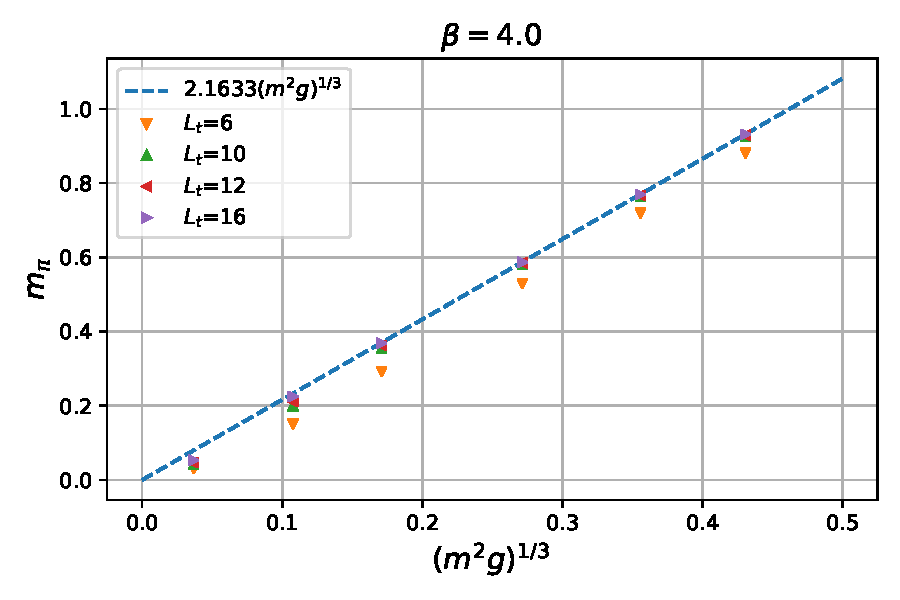
\includegraphics[width=1\textwidth]{figs/FiniteTMPiHos}
\end{frame}

\begin{frame}{Pion mass - Hosotani vs. lattice simulation}
  \includegraphics[width=1\textwidth]{figs/MPi64x10FiniteT}
\end{frame}

\begin{frame}{Pion mass - Hosotani vs. lattice simulation}
  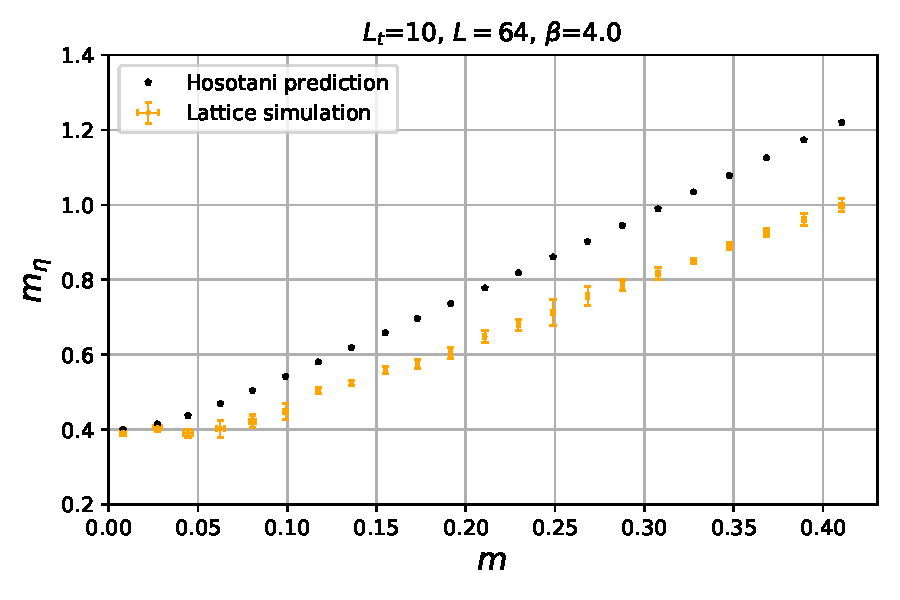
\includegraphics[width=1\textwidth]{figs/Meta64x10FiniteT}
\end{frame}


\section{$\delta$-regime}

\begin{frame}{$\delta$-regime}
  \begin{itemize}
    \item spatial volume is small compared to the correlation
      length
      \[
        \xi = m_\pi^{-1}
      \]
      but the Euclidean time extent is large
      \[
        L_t\gg \xi \gtrsim L
      \]
    \item the system is quasi one dimensional - approximation by
      quantum rotor [Leutwyler, 1987]
    \item pion has \textit{residual mass}
      \[
        m_\pi^R = \frac{3}{2\Theta}
      \]
      where $\Theta$ is the moment of inertia
  \end{itemize}
\end{frame}

\begin{frame}{Residual pion mass plateau: $L_t = 64, L = 10$}
  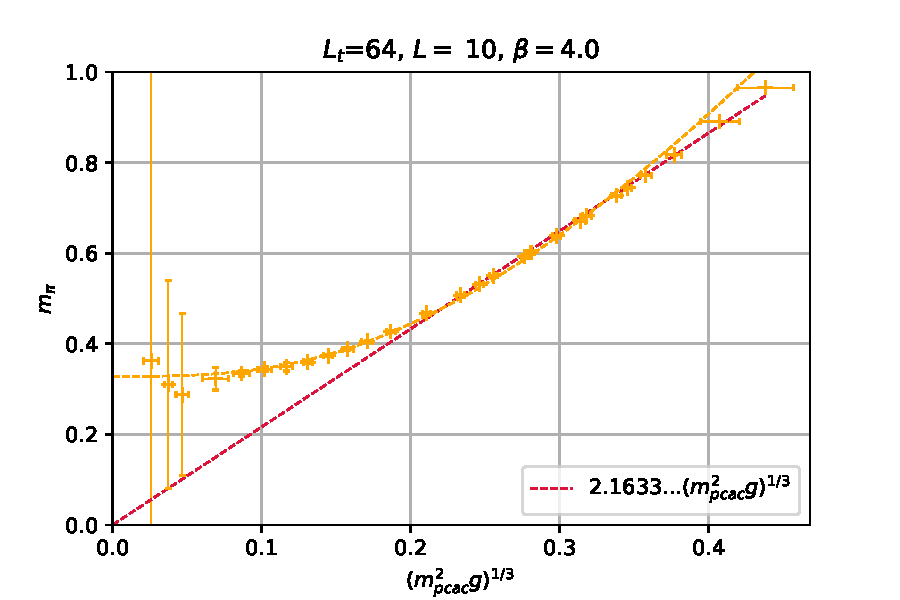
\includegraphics[width=1\textwidth]{figs/Mpi10x64}
\end{frame}

\begin{frame}{Residual pion mass plateau: $L_t = 64, L = 6$}
  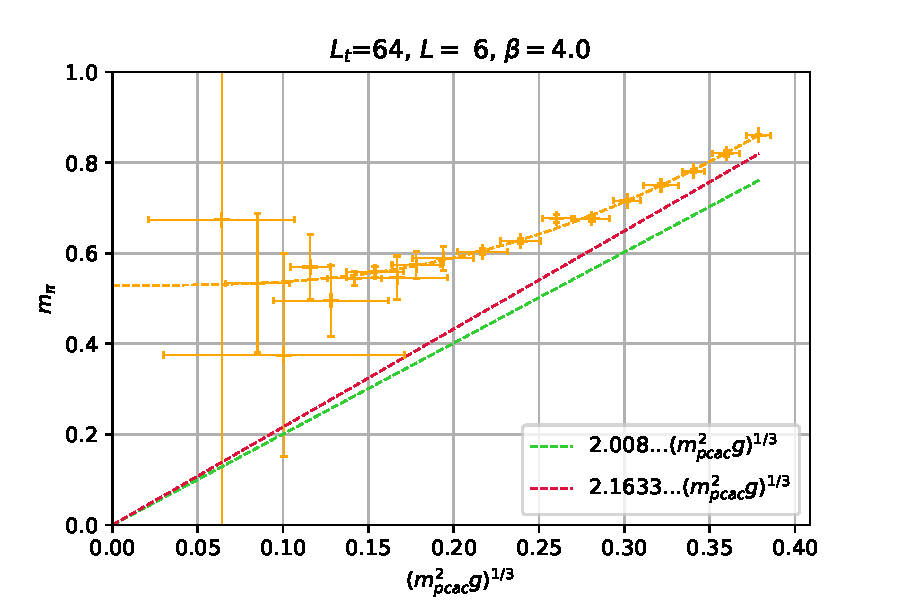
\includegraphics[width=1\textwidth]{figs/Mpi6x64Pt10}
\end{frame}

\begin{frame}{Conjecture}
  \begin{itemize}
    \item {[Hasenfratz and Niedermayer, 1993]} computed $\Theta$
      up to next-to-leading order, for a general dimension $d > 2$
            \[
        \Theta = F_\pi^2 L^{d-1} \left[1 +
          \frac{\cal{N} - 2}{4\pi F_\pi^2 L^{d-2}}
          \left(2\frac{d - 1}{d - 2} + ...\right) \right]
      \]
    \item in two dimensions ($d = 2$) there is a divergence of 
      the next to leading term, so we just consider the 
      leading term
      \[
        m_\pi^R \simeq \frac{3}{2F_\pi^2 L}
      \]
    \item we verify the relation $m_\pi^R \propto 1 / L$ with
      simulation data and extract the value of pion decay
      constant $F_\pi$
  \end{itemize}
\end{frame}

\begin{frame}{1 / L confirmed by lattice simulation}
  \begin{columns}[t]
    \column{0.5\textwidth}
      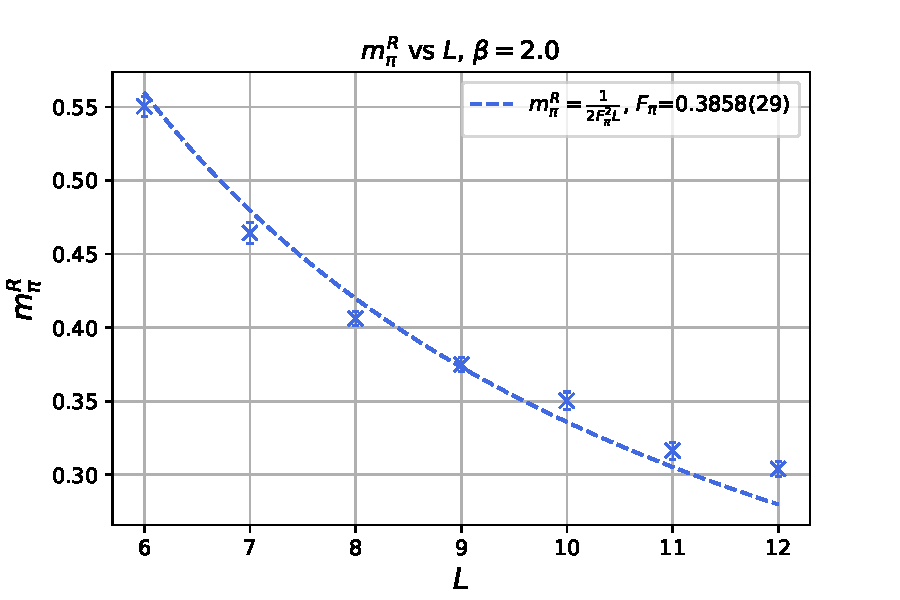
\includegraphics[width=1.0\textwidth]{figs/ResMpiBeta2}
      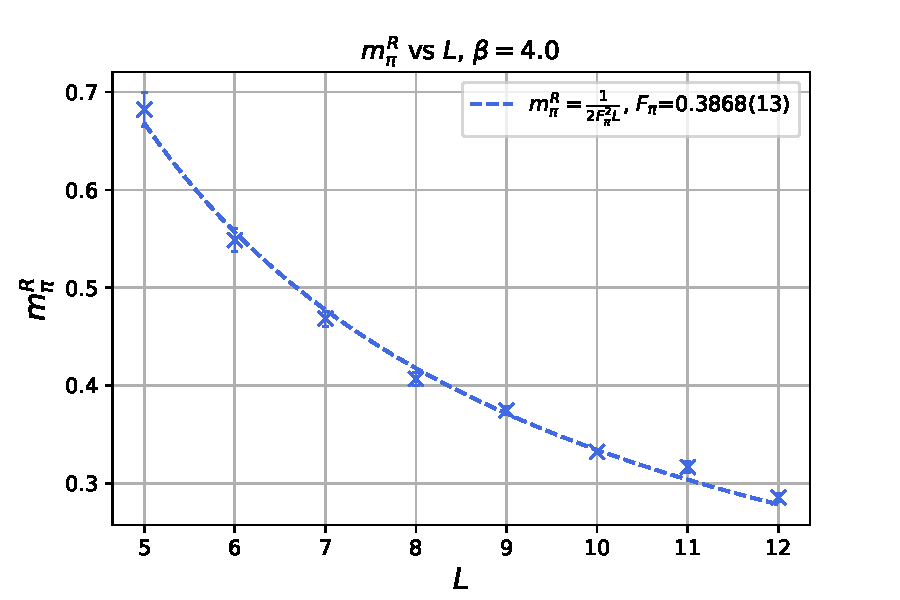
\includegraphics[width=1.0\textwidth]{figs/ResMpiBeta4}
    \column{0.5\textwidth}
      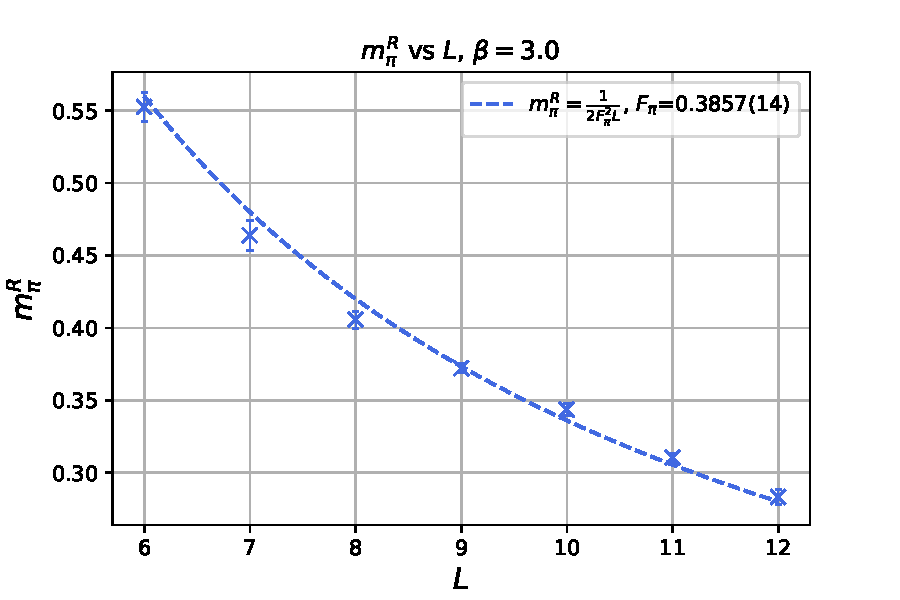
\includegraphics[width=1.0\textwidth]{figs/ResMpiBeta3}
      \begin{center} 
	    \begin{tabular}{c c c c}
	      $\beta$ & $F_\pi$ \\
	      \hline
	      2.0 & 0.6683(50) \\
	      \hline
	      3.0 & 0.6681(25) \\
	      \hline
	      4.0 & 0.6700(22) \\
	    \end{tabular}
        \[
      	  F_\pi = 0.6688(5)
        \]
      \end{center}	 
  \end{columns}
\end{frame}


\section{Witten-Veneziano}

\begin{frame}{Witten-Veneziano formula}
  \begin{itemize}
    \item in the chiral $N$-flavor Schwinger model the
      Witten-Veneziano formula is simplified to [Seiler and
      Stamatescu, 1987]
      \[
        m_\eta^2 = \frac{2N}{F_\eta^2}\chi_T^{que}
      \]
    \item mass of the $\eta$ particle is known analytically
      [Belvedere et al., 1979] 
      \[
        m_\eta^2 = \frac{N}{\pi\beta}
      \]
    \item continuum prediction for $\chi_T^{que}$
      [Seiler and Stamatescu, 1987]
      \[
        \beta\chi_T^{que} = \frac{1}{4\pi^2}
      \]
  \end{itemize}
\end{frame}

\begin{frame}{Quenched topological susceptibility}
  \begin{itemize}
    \item {[Bardeen et al., 1998]} were able to analytically
      compute $\chi_T^{que}$ on the lattice
      \[
        \beta\chi_T^{que} = \frac{I_1(\beta)}{4 \pi^2 I_0(\beta)}
      \]
      by using an alternative definition of topological charge
      \[
        Q_S = \frac{1}{2\pi}\sum_{P}\sin(\theta_P)
      \]
    \item for the usual definition of topological charge
      \[
        Q_T = \frac{1}{2\pi}\sum_{P}\theta_P
      \]
      it is not possible to find analytic expression, but using the 
      same line of reasoning it is possible to numerically compute
      $\chi_T^{que}$ to arbitrary precision
  \end{itemize}
\end{frame}

\begin{frame}{Quenched topological susceptibility}
  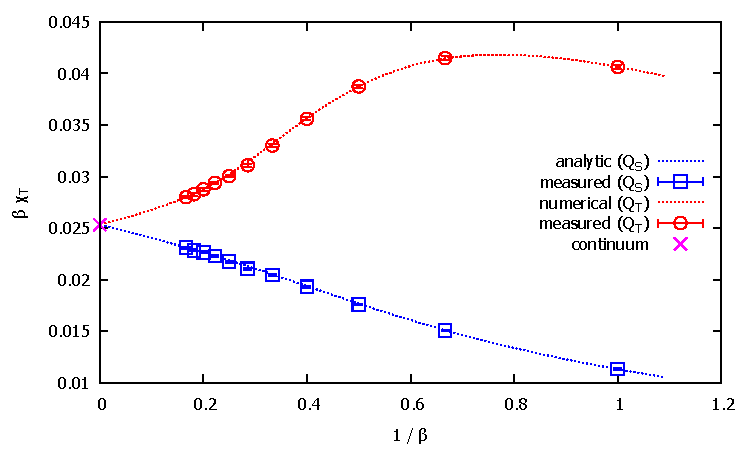
\includegraphics[width=1\textwidth]{figs/BeakDiagram}
\end{frame}

\begin{frame}{$F_\eta$ versus $F_\pi$}
\begin{itemize}
  \item in large $N_c$ QCD, to the order $1/N_c$
    \[
      F_{\eta'} = F_\pi
    \]
  \item in the Schwinger model nothing assures that this relation holds
  \item inserting the confirmed values for $m_\eta^2$ and $\chi_T^{que}$ 
    \[
      F_{\eta}^2 = \frac{2N}{m_\eta^2}\chi_T^{que} =
        2N \left(\frac{\pi\beta}{N}\right)
        \left(\frac{1}{4\pi^2\beta}\right) =
        \frac{1}{2\pi}
    \]
  \item our results suggest that in the Schwinger model these two decay constants differ significantly
    \[
      F_{\eta} = 0.3989 \qquad F_\pi = 0.6688(5)
    \]
\end{itemize}
\end{frame}

\end{document}
